\section{Dataset and Demand Construction}

\subsection{Intended Dartmouth Dataset}

The intended real-world source is the CRAWDAD Dartmouth campus WLAN dataset. The current official Dartmouth page describes the 2009 release as containing more than five years of syslog, SNMP, and tcpdump traces from a campus deployment with more than 450 APs and several thousand users \cite{kotz_dartmouth_campus_2009}. Earlier Dartmouth releases and studies have been widely used for AP-level WLAN mobility modeling \cite{Kotz2004Dartmouth,kim2005mobility_wifi_ap}.

At the time of this study, legacy direct CRAWDAD movement-trace URLs were unavailable through unauthenticated download, while the official page points to IEEE DataPort. We therefore record the official source pages and an access note under \texttt{data/raw/dartmouth\_access/}. The raw dataset is not redistributed.

\subsection{Trace-Compatible Fallback}

To keep the experimental pipeline executable, we provide a deterministic trace-compatible mobility file saved as \texttt{data/raw/dartmouth\_movement.csv}. It has columns \texttt{user\_id}, \texttt{timestamp}, and \texttt{ap}. A sidecar metadata file marks it as synthetic. The generator simulates users moving among AP clusters, occasionally entering an \texttt{OFF} state, and producing ordered AP association sequences.

This generated movement file is not claimed to be the Dartmouth raw trace. It is a reproducibility device that allows the complete graph-construction, caching, and evaluation pipeline to run when the raw archive is unavailable.

The trace-compatible generator is deterministic for a fixed seed. Mobile clients are assigned to AP communities, remain mostly within a home community, occasionally move to neighboring communities, and sometimes disconnect through the \texttt{OFF} state. This creates community structure and nonuniform handoff counts, two properties needed for meaningful graph-aware caching evaluation.

\subsection{Preprocessing}

Records are sorted by user and timestamp. \texttt{OFF} intervals are removed before graph construction because they represent absence from the WLAN. Consecutive AP changes define handoffs. For each user sequence \(i_1,i_2,\ldots,i_T\), each transition \(i_t\rightarrow i_{t+1}\) with \(i_t\ne i_{t+1}\) increments handoff count \(H_{i_t,i_{t+1}}\). The implementation selects the most active APs and keeps the largest connected component.

\begin{table}[t]
\centering
\caption{Dataset and graph statistics for the final reproducible run.}
\label{tab:dataset_stats}
\begin{tabular}{lr}
\toprule
Property & Value \\
\midrule
Movement records & 25,600 \\
Selected AP nodes & 20 \\
Weighted mobility edges & 190 \\
Content catalog size & 48 \\
Cache capacity per node & 5 objects \\
Zipf skew parameter \(\alpha\) & 0.85 \\
Spatial locality multiplier & 2.8 \\
Trace-compatible generated mobility used & Yes \\
\bottomrule
\end{tabular}
\end{table}

\begin{figure}[t]
\centering
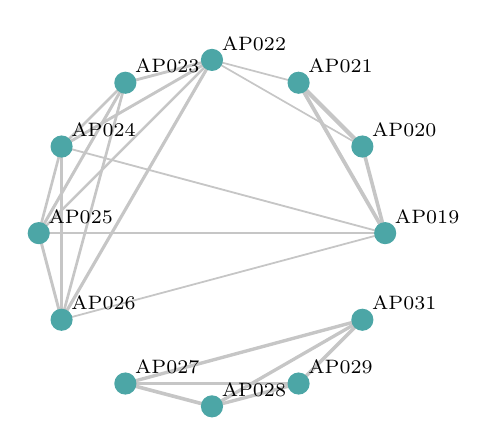
\begin{tikzpicture}[x=1cm,y=1cm, every node/.style={font=\scriptsize}]
\draw[gray!45, line width=1.50pt] (1.91,1.10) -- (1.10,1.91);
\draw[gray!45, line width=1.36pt] (2.20,0.00) -- (1.10,1.91);
\draw[gray!45, line width=1.31pt] (-1.10,-1.91) -- (-0.00,-2.20);
\draw[gray!45, line width=1.31pt] (1.10,-1.91) -- (1.91,-1.10);
\draw[gray!45, line width=1.30pt] (2.20,0.00) -- (1.91,1.10);
\draw[gray!45, line width=1.22pt] (-0.00,-2.20) -- (1.10,-1.91);
\draw[gray!45, line width=1.22pt] (-1.10,-1.91) -- (1.91,-1.10);
\draw[gray!45, line width=1.20pt] (-0.00,-2.20) -- (1.91,-1.10);
\draw[gray!45, line width=1.20pt] (-1.10,-1.91) -- (1.10,-1.91);
\draw[gray!45, line width=1.14pt] (0.00,2.20) -- (-1.91,-1.10);
\draw[gray!45, line width=1.09pt] (-1.10,1.91) -- (-2.20,0.00);
\draw[gray!45, line width=1.06pt] (-2.20,0.00) -- (-1.91,-1.10);
\draw[gray!45, line width=1.05pt] (-1.91,1.10) -- (-1.91,-1.10);
\draw[gray!45, line width=1.05pt] (0.00,2.20) -- (-1.91,1.10);
\draw[gray!45, line width=1.03pt] (0.00,2.20) -- (-1.10,1.91);
\draw[gray!45, line width=0.97pt] (-1.10,1.91) -- (-1.91,-1.10);
\draw[gray!45, line width=0.96pt] (-1.91,1.10) -- (-2.20,0.00);
\draw[gray!45, line width=0.95pt] (-1.10,1.91) -- (-1.91,1.10);
\draw[gray!45, line width=0.95pt] (0.00,2.20) -- (-2.20,0.00);
\draw[gray!45, line width=0.66pt] (2.20,0.00) -- (-1.91,1.10);
\draw[gray!45, line width=0.64pt] (2.20,0.00) -- (-1.91,-1.10);
\draw[gray!45, line width=0.62pt] (2.20,0.00) -- (-2.20,0.00);
\draw[gray!45, line width=0.62pt] (1.10,1.91) -- (0.00,2.20);
\draw[gray!45, line width=0.61pt] (1.91,1.10) -- (0.00,2.20);
\fill[teal!70] (2.20,0.00) circle (4pt);
\node[above right] at (2.20,0.00) {AP019};
\fill[teal!70] (1.91,1.10) circle (4pt);
\node[above right] at (1.91,1.10) {AP020};
\fill[teal!70] (1.10,1.91) circle (4pt);
\node[above right] at (1.10,1.91) {AP021};
\fill[teal!70] (0.00,2.20) circle (4pt);
\node[above right] at (0.00,2.20) {AP022};
\fill[teal!70] (-1.10,1.91) circle (4pt);
\node[above right] at (-1.10,1.91) {AP023};
\fill[teal!70] (-1.91,1.10) circle (4pt);
\node[above right] at (-1.91,1.10) {AP024};
\fill[teal!70] (-2.20,0.00) circle (4pt);
\node[above right] at (-2.20,0.00) {AP025};
\fill[teal!70] (-1.91,-1.10) circle (4pt);
\node[above right] at (-1.91,-1.10) {AP026};
\fill[teal!70] (-1.10,-1.91) circle (4pt);
\node[above right] at (-1.10,-1.91) {AP027};
\fill[teal!70] (-0.00,-2.20) circle (4pt);
\node[above right] at (-0.00,-2.20) {AP028};
\fill[teal!70] (1.10,-1.91) circle (4pt);
\node[above right] at (1.10,-1.91) {AP029};
\fill[teal!70] (1.91,-1.10) circle (4pt);
\node[above right] at (1.91,-1.10) {AP031};
\end{tikzpicture}
\caption{Mobility-derived AP handoff graph sample generated from the trace-compatible movement data. Edge thickness reflects relative handoff count among the strongest displayed links.}
\label{fig:generated_mobility_graph}
\end{figure}


\subsection{Synthetic Content Demand}

Because the movement trace does not contain content request identities, demand is synthesized. Global popularity follows a Zipf distribution:
\[
p_r=\frac{r^{-\alpha}}{\sum_{k=1}^{M} k^{-\alpha}},
\]
where \(r\) is content rank, \(M\) is catalog size, and \(\alpha\) controls skew. Node-level demand then applies an AP-cluster locality multiplier and renormalizes the distribution. This produces correlated but non-identical demand across neighboring APs, which is necessary for evaluating redundancy and diversity.

The model separates two signals. Global popularity captures the fact that a few objects are requested much more often than most objects. Spatial locality captures the fact that different APs or buildings may have different dominant interests. Without locality, global top-\(K\) caching would be unrealistically strong. Without global popularity, the workload would not reflect content-delivery systems. The Zipf-locality mixture gives a controlled middle ground.

\begin{table}[t]
\centering
\caption{Dataset artifacts produced by the implementation.}
\label{tab:data_artifacts}
\begin{tabular}{p{0.38\textwidth}p{0.48\textwidth}}
\toprule
Artifact & Purpose \\
\midrule
\texttt{data/raw/dartmouth\_access/ACCESS\_NOTE.txt} & Documents official dataset access constraints. \\
\texttt{data/raw/dartmouth\_movement.csv} & Trace-compatible movement data used by the executable pipeline. \\
\texttt{data/raw/dartmouth\_movement.csv.metadata.json} & Marks whether the movement file is generated trace-compatible data. \\
\texttt{results/final/run\_metadata.json} & Records graph size, configuration, runtime, and generated-data status. \\
\bottomrule
\end{tabular}
\end{table}
